\documentclass[a4paper]{article}

\usepackage[utf8]{inputenc}
\usepackage[T2A]{fontenc}
\usepackage[russian]{babel}

\usepackage{mathtext}

\usepackage{listings}
\usepackage{color}

\definecolor{mygreen}{rgb}{0,0.6,0}
\definecolor{mygray}{rgb}{0.5,0.5,0.5}
\definecolor{mymauve}{rgb}{0.58,0,0.82}

\lstset{
	morekeywords={*,...}, % если хотите добавить ключевые слова
	keywordstyle=\color{blue},
	stringstyle=\color{mymauve},
	% Настройки отображения
	breaklines=true, % Перенос длинных строк
	basicstyle=\footnotesize, % Шрифт для отображения кода
	backgroundcolor=\color{white}, % Цвет фона кода
	frame=single,
	rulecolor=\color{black}, % Цвет рамки
	tabsize=3, % Размер табуляции в пробелах
	% Настройка отображения номеров строк. Если не нужно, то удалите весь блок
	numbers=left, % Слева отображаются номера строк
	stepnumber=1, % Каждую строку нумеровать
	numbersep=5pt, % Отступ от кода
	numberstyle=\tiny\color{mygray},
	% Для отображения русского языка
	extendedchars=true,
	literate={Ö}{{\"O}}1
	{Ä}{{\"A}}1
	{Ü}{{\"U}}1
	{ß}{{\ss}}1
	{ü}{{\"u}}1
	{ä}{{\"a}}1
	{ö}{{\"o}}1
	{~}{{\textasciitilde}}1
	{а}{{\selectfont\char224}}1
	{б}{{\selectfont\char225}}1
	{в}{{\selectfont\char226}}1
	{г}{{\selectfont\char227}}1
	{д}{{\selectfont\char228}}1
	{е}{{\selectfont\char229}}1
	{ё}{{\"e}}1
	{ж}{{\selectfont\char230}}1
	{з}{{\selectfont\char231}}1
	{и}{{\selectfont\char232}}1
	{й}{{\selectfont\char233}}1
	{к}{{\selectfont\char234}}1
	{л}{{\selectfont\char235}}1
	{м}{{\selectfont\char236}}1
	{н}{{\selectfont\char237}}1
	{о}{{\selectfont\char238}}1
	{п}{{\selectfont\char239}}1
	{р}{{\selectfont\char240}}1
	{с}{{\selectfont\char241}}1
	{т}{{\selectfont\char242}}1
	{у}{{\selectfont\char243}}1
	{ф}{{\selectfont\char244}}1
	{х}{{\selectfont\char245}}1
	{ц}{{\selectfont\char246}}1
	{ч}{{\selectfont\char247}}1
	{ш}{{\selectfont\char248}}1
	{щ}{{\selectfont\char249}}1
	{ъ}{{\selectfont\char250}}1
	{ы}{{\selectfont\char251}}1
	{ь}{{\selectfont\char252}}1
	{э}{{\selectfont\char253}}1
	{ю}{{\selectfont\char254}}1
	{я}{{\selectfont\char255}}1
	{А}{{\selectfont\char192}}1
	{Б}{{\selectfont\char193}}1
	{В}{{\selectfont\char194}}1
	{Г}{{\selectfont\char195}}1
	{Д}{{\selectfont\char196}}1
	{Е}{{\selectfont\char197}}1
	{Ё}{{\"E}}1
	{Ж}{{\selectfont\char198}}1
	{З}{{\selectfont\char199}}1
	{И}{{\selectfont\char200}}1
	{Й}{{\selectfont\char201}}1
	{К}{{\selectfont\char202}}1
	{Л}{{\selectfont\char203}}1
	{М}{{\selectfont\char204}}1
	{Н}{{\selectfont\char205}}1
	{О}{{\selectfont\char206}}1
	{П}{{\selectfont\char207}}1
	{Р}{{\selectfont\char208}}1
	{С}{{\selectfont\char209}}1
	{Т}{{\selectfont\char210}}1
	{У}{{\selectfont\char211}}1
	{Ф}{{\selectfont\char212}}1
	{Х}{{\selectfont\char213}}1
	{Ц}{{\selectfont\char214}}1
	{Ч}{{\selectfont\char215}}1
	{Ш}{{\selectfont\char216}}1
	{Щ}{{\selectfont\char217}}1
	{Ъ}{{\selectfont\char218}}1
	{Ы}{{\selectfont\char219}}1
	{Ь}{{\selectfont\char220}}1
	{Э}{{\selectfont\char221}}1
	{Ю}{{\selectfont\char222}}1
	{Я}{{\selectfont\char223}}1
	{і}{{\selectfont\char105}}1
	{ї}{{\selectfont\char168}}1
	{є}{{\selectfont\char185}}1
	{ґ}{{\selectfont\char160}}1
	{І}{{\selectfont\char73}}1
	{Ї}{{\selectfont\char136}}1
	{Є}{{\selectfont\char153}}1
	{Ґ}{{\selectfont\char128}}1
	{\{}{{{\color{black}\{}}}1 % Цвет скобок {
	{\}}{{{\color{black}\}}}}1 % Цвет скобок }
	,
%	title=\lstname
}

\usepackage{algorithmicx}
\usepackage{algpseudocode}

\usepackage{amssymb}
\usepackage{amsopn}
\usepackage{mathtools}

\usepackage{graphicx}

\usepackage[
a4paper, includefoot,
left=2cm, right=1cm, top=2cm, bottom=2cm,
]{geometry}

\usepackage[hidelinks]{hyperref}
\usepackage{multirow}
\usepackage{cmap}


\begin{document}

\begin{titlepage}

	\begin{center}

		\large Федеральное государственное автономное образовательное учреждение высшего образования \\
		\large «Санкт-Петербургский политехнический университет Петра Великого» \\
		\large Институт компьютерных наук и технологий \\
		\large Кафедра «Компьютерные интеллектуальные технологии» \\[4cm]

		\huge {\bf Курсовая работа} \\[0.5cm]
		\large {\bf Информационная система автомобилестроительного предприятия} \\[0.1cm]
		\large по дисциплине «Базы данных» \\[4cm]

	\end{center}

    \begin{center}
        \begin{minipage}[t]{4cm}
            \begin{flushleft}
                Выполнил студент гр. 23506/1
            \end{flushleft}
        \end{minipage}
        \hfill
        \begin{minipage}[t]{4cm}
            \begin{flushright}
            О.Д. Романов
            \end{flushright}
        \end{minipage} \\[0.5cm]

        \begin{minipage}[t]{4cm}
            \begin{flushleft}
                Руководитель старший преподаватель
            \end{flushleft}
            \flushleft
        \end{minipage}
        \hfill
        \begin{minipage}[t]{4cm}
            \begin{flushright}
                Н.В. Андреева
            \end{flushright}
        \end{minipage}
    \end{center}

    \begin{flushright}
        14 мая 2017
    \end{flushright}

	
	\vfill

	\begin{center}
	    \large Санкт-Петербург\\
	    \large \the\year
	\end{center}
 
\end{titlepage}

\tableofcontents
\newpage

\section{Исходные данные}

\subsection{Техническое задание}
Структурно предприятие состоит из цехов, которые в свою очередь подразделяются на участки.

Категории изделий, выпускаемых предприятием: грузовые, легковые автомобили, автобусы, сельскохозяйственные, дорожно-строительные машины, мотоциклы и прочие изделия.
Каждая категория изделий имеет специфические, присущие только ей атрибуты.
Например, для автобусов это вместимость, для сельскохозяйственных и дорожно-строительных машин - производительность и т.д.

По каждой категории изделий может собираться несколько видов изделий (под видом изделия понимается конкретная его разновидность / марка - например, автомобиль KIA Rio).
По конкретным экземплярам каждого вида ведётся журнал, где отмечаются даты завершения различных этапов жизненного цикла изделия: изготовление (сборка) / тестирование / передача дилеру / гарантийный ремонт.

Предприятие в основном состоит из производственных цехов, но также есть несколько вспомогательных (например, ремонтный, тестировочный).

Каждая категория изделий собирается в своём производственном цехе (в одном цехе может собираться несколько категорий изделий).
Цех структурно состоит из участков, на каждом из которых выполняется один вид работ: изготавливается определённая часть изделия (например, двигатель) либо производится сборка изделия в целом.
С каждой категорией изделия ассоциируется свой набор работ; другими словами, каждая категория в процессе изготовления должна пройти определённый набор участков в цехе.

Каждой категории инженерно-технического персонала (инженеры, технологи, техники) и рабочих (сборщики, токари, слесари, сварщики и пр.) также характерны атрибуты, свойственные только для этой группы.
Рабочие объединяются в бригады, которыми руководят бригадиры.
Бригадиры выбираются из числа рабочих.
Работу цеха возглавляет начальник цеха, а работу на участке - начальник участка, в подчинении которого находится несколько мастеров.
Каждый мастер координирует работу одной или нескольких бригад (но, в отличие от бригадира, не входит в состав конкретной бригады).
Мастера, начальники участков и цехов назначаются из числа инженерно-технического персонала.
Каждый начальник может руководить только одной структурной единицей (в т.ч. начальник одной структурной единицы не может быть в то же время начальником другой).

Работу по сборке конкретной категории изделия на определенном участке выполняет одна бригада рабочих, при этом она может обслуживать несколько участков / категорий и на одном участке может работать несколько бригад.

\subsection{Виды запросов в информационной системе}
\begin{enumerate}

    \item Перечень видов изделий по категории, собираемой указанным цехом.
    В последней строке вывести общее число собираемых видов изделий.

    \item Количество экземпляров изделий каждого вида каждой категории, собранных предприятием за определенный отрезок времени.
    В последней строке вывести общее число собранных изделий.
    Примерный вид результата:

    \begin{tabular}{|p{6cm}|p{2cm}|p{1cm}|} \hline
        Категория & Вид & Кол-во \\ \hline
        Автобусы & АКБ-12 & 8 \\ \hline
        Автобусы & АКБ-05 & 0 \\ \hline
        Автомобили & ИЖ-400 & 12 \\ \hline
        ... & ... & ... \\ \hline
        Всего собрано (12.05.2010-18.07.2010): & & 48 \\ \hline
    \end{tabular}

    \item Данные о кадровом составе (ФИО, должность) по указанным категориям инженерно-технического персонала и рабочих;
    \item Число и перечень участков предприятия и их начальников (с указанием цехов).
    \item Перечень работ, которые проходит указанный вид изделия.
    \item Состав бригад, работающих на указанном участке указанного цеха: ФИО рабочего, номер бригады, номер участка, номер цеха. Отсортировать по номеру бригады.
    \item Перечень мастеров (ФИО) указанного участка указанного цеха и номера бригад, работы которых они координируют.
    \item Информация о цехах, в которых в настоящий момент собирается больше видов изделий, чем в среднем приходится на каждый производственный цех предприятия: номер цеха, название цеха, кол-во собираемых видов изделий, среднее количество видов изделий по цехам предприятия.
    \item Состав бригад, участвующих в сборке указанной категории изделия.
    \item ФИО и должности работников цеха, в котором собирается больше всего категорий изделий.

\end{enumerate}

\section{Сущности, их харрактеристики и связи}
В ходе анализа начального описания предметной области были выявлены следующие сущности:

\begin{enumerate}

    \item Сотрудник

    Базовая сущность сотрудника, которая содержит информацию о его фамилии (not null), его имени (not null), номере договора (PK), отчестве (nullable) и типе сотрудника (ИТП или Рабочий).

    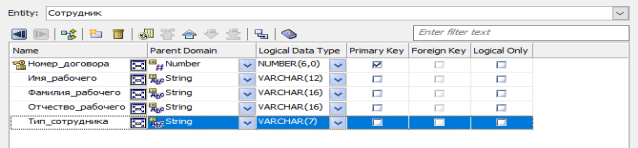
\includegraphics[height=3cm]{screenshots/entities/employee.png}

    \item ИТП

    Инженерно-технический персонал. С помощью категориальной связи соеденим Сотрудника (супертип) и ИТП (подтип).
    Содержит информацию о номере договра и FK на категорию ИТП

    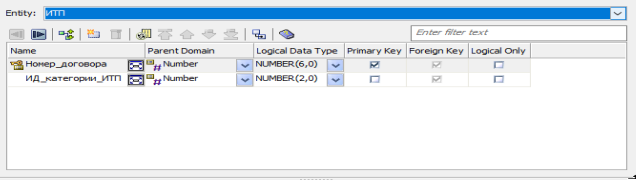
\includegraphics[height=3cm]{screenshots/entities/itp.png}

    \item Категория ИТП

    Категории инженерно-технический персонал (инженеры, техники, технологи).
    С помощью связи один ко многим соеденим ИТП и Категория\_ИТП.
    Причем, ИТП должен соответствовать одна категория, а категория может не быть у какого-то ИТП.

    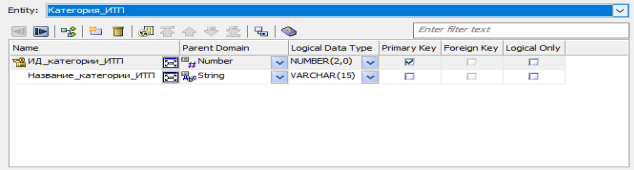
\includegraphics[height=3cm]{screenshots/entities/category_itp.png}

    \item Атрибуты ИТП

    Категории инженерно-технический персонал (инженеры, техники, технологи).
    С помощью связи многие ко многим соеденим Категория\_ИТП и Атрибуты\_ИТП.
    У каждой категории может быть несколько атрибутов и атрибут может быть в нескольких категориях.

    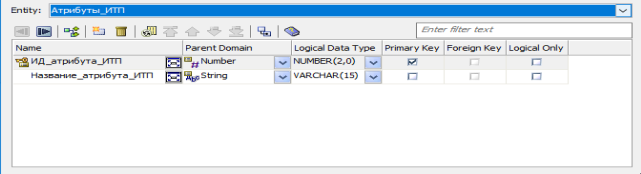
\includegraphics[height=3cm]{screenshots/entities/attribute_itp.png}

    \item Рабочий

    С помощью категориальной связи соеденим Сотрудника (супертип) и Рабочий (подтип).
    Содержит информацию о номере договра, категории рабочего и бригаде, в которой он состоит.

    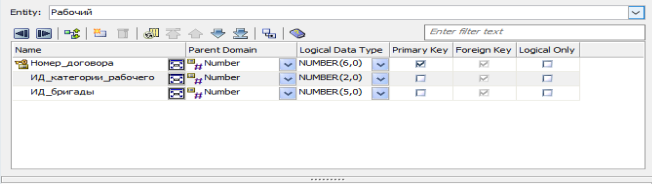
\includegraphics[height=3cm]{screenshots/entities/worker.png}

    \item Категория рабочего

    Содержит информацию о категории рабочего: название категории и ее идентификатор.

    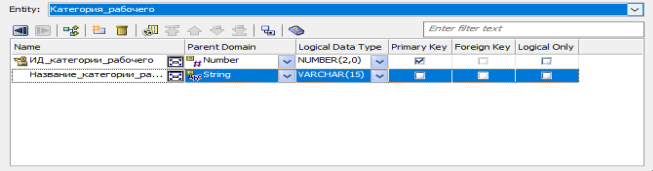
\includegraphics[height=3cm]{screenshots/entities/category_worker.png}

    \item Атрибуты рабочего

    С помощью связи многие ко многим соеденим Категория\_рабочего и Атрибуты\_рабочего.
    У каждой категории может быть несколько атрибутов и атрибут может быть в нескольких категориях.

    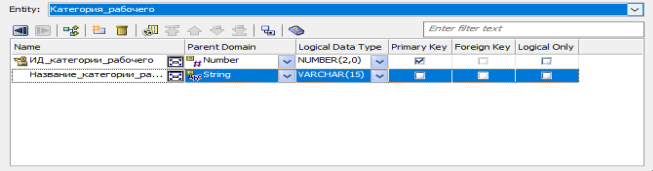
\includegraphics[height=3cm]{screenshots/entities/category_worker.png}

    \item Бригада

    Информация о бригаде.
    Как-то не очень!!!

    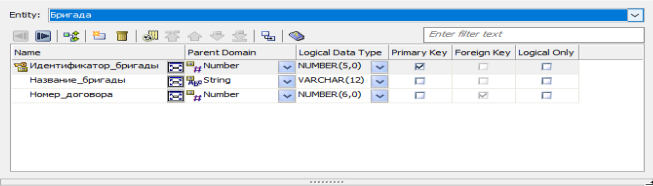
\includegraphics[height=3cm]{screenshots/entities/bad_workers_crew.png}

    \item Мастер

    \item Начальник участка

    \item Начальник цеха

    \item Начальник мастер

    \item Участок

    \item Цех

    \item Журнал

    \item Вид изделия

    \item Категория изделия

    \item Атрибуты изделия

    \item Вид работы

    \item КатИздВидРаботы

\end{enumerate}


\section {Нормализация}

\section {ERwin Data Model Validator}

\section {Реализация запросов к базе данных}

\end{document}